\important{Focus sur: la centrale nucléaire}

\begin{center}
    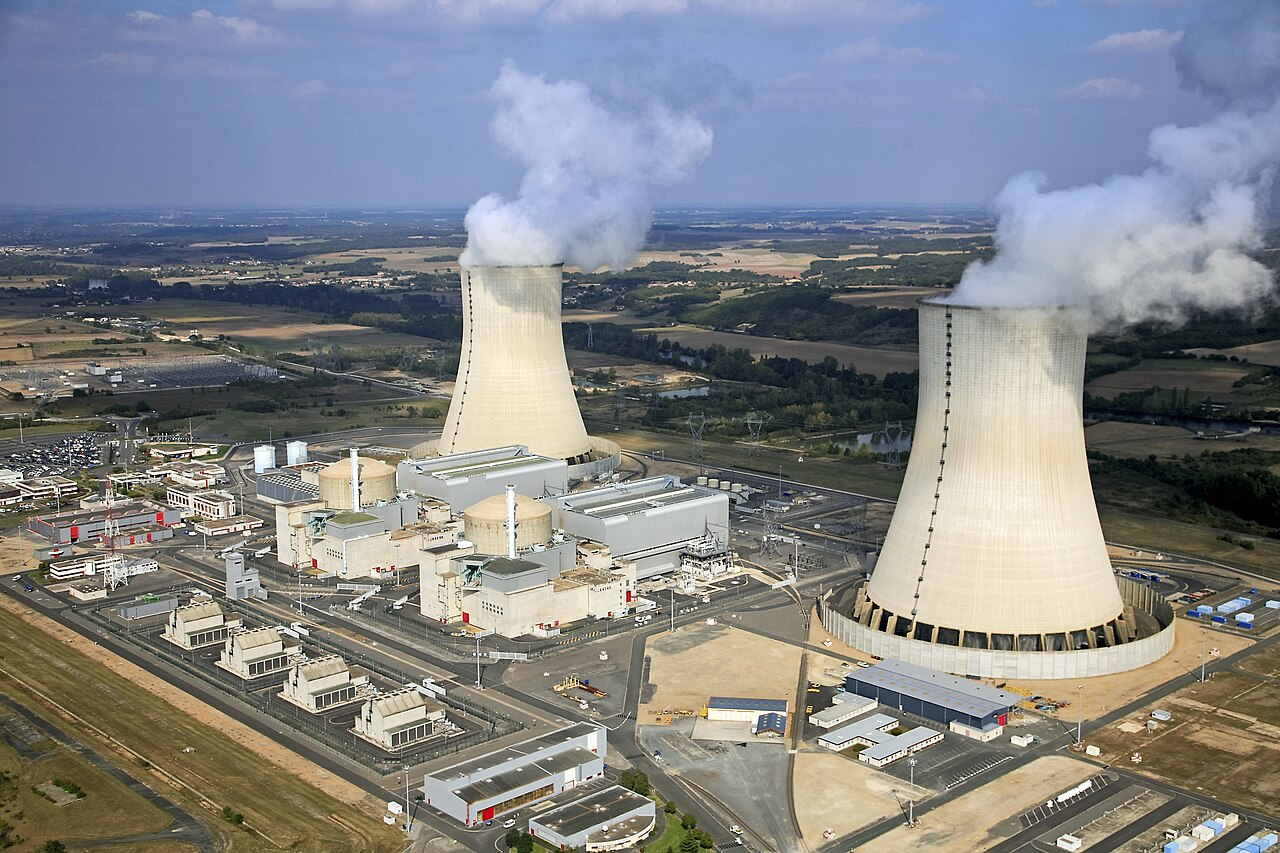
\includegraphics[width=6cm]{images/nucleaire.JPG}

    \textit{Centrale nucléaire de Civaux (Vienne)}
\end{center}


Une centrale nucléaire est un dispositif qui permet de produire de l'électricité à partir d'un combustible appelé uranium. L'uranium subit une réaction nucléaire qui libère une énorme quantité de chaleur.
Cette chaleur sert à chauffer de l'eau pour la transformer en vapeur. La vapeur fait alors tourner une turbine, qui entraîne un alternateur produisant de l'électricité.
Les grandes tours ne sont pas des cheminées : ce sont des tours de refroidissement qui rejettent uniquement de la vapeur d'eau, et non de la fumée polluante.

La centrale nucléaire utilise l'uranium, une source d'énergie non renouvelable, mais elle ne rejette pas de CO\textsubscript{2}. Sa production est très forte et continue jour et nuit.
Cependant, le fonctionnement d'un réacteur produit des déchets radioactifs dangereux, qu'il faut stocker pendant des milliers d'années. Il existe aussi un risque d'accident nucléaire.